\documentclass{book}
\usepackage[utf8]{inputenc}
\usepackage[spanish]{babel}
\usepackage{graphicx}
\usepackage{graphicx, subfigure}
\usepackage{mathptmx}
\usepackage{multicol}
\usepackage{color}
\usepackage{listings}
\usepackage[square,authoryear]{natbib}
\bibliographystyle{dinat}
\usepackage[usenames,dvipsnames,svgnames,table]{xcolor}

\addto\captionsspanish{\renewcommand{\contentsname}{CONTENIDO}}

\begin{document}
	\thispagestyle{empty}
	\frontmatter
	\begin{minipage}{.3\textwidth}
	\begin{flushleft}
		\begin{center}
			{
\includegraphics[scale=.35]{Assets/images/escudo_unam.png}}
		\end{center}
		\vspace{10pt}
		\begin{center}{
				\rule{.5pt}{.6\textheight}
				\hspace{7pt}
				\rule{2pt}{.6\textheight}
				\hspace{7pt}
				\rule{.5pt}{.6\textheight}
			}
		\end{center}
		\begin{center}{
\includegraphics[scale=1]{Assets/images/escudo_fi.jpg}}\end{center}
	\end{flushleft}
	\end{minipage}
	\begin{minipage}{.7\textwidth}
		\begin{flushright}
				\begin{center}
				\begin{center}
					\LARGE{U}\large{NIVERSIDAD} \LARGE{N}\large{ACIONAL} 
					\LARGE{A}\large{UTÓNOMA} \\[10pt]
					\large{DE} 
					\LARGE{M}\large{ÉXICO} 
				\end{center}
				\rule{\textwidth}{2pt}
				\\
				\hrulefill\\[1cm]
				
				\LARGE{F}\large{ACULTAD DE } \LARGE{I}\large{NGENIERÍA}\\[2cm]
				
				\large{Diseño e implementación de un entorno computacional para la ayuda en la síntesis de sonidos musicales}\\[1.5cm]
				
				\huge{T E S I S }\\[1.5cm]
				
				\large{QUE PARA OBTENER EL TÍTULO DE:}\\[1cm]
				
				\large{INGENIERO EN COMPUTACIÓN}\\[1cm]
				
				\large{PRESENTA}
				
				\large{Joaquín Gustavo Espino de Horta}\\[1cm]
				
				\large{DIRECTOR DE TESIS}
				
				\large{Dr. Rogelio Alcántara Silva}\\[1cm]
				
				\large{Ciudad Universitaria, Cd. Mx., Agosto 2024}
				
			\end{center}
		\end{flushright}
	\end{minipage}
	
	\section*{Agradecimientos}
	Tras muchos años en pie de lucha contra las adversidades internas y externas, finalmente puedo tomarme un respiro para mirar atrás, me sorprende la cantidad exacta del tiempo tomado hasta este punto, tan corta para ser toda mi historia y mucha para ignorar su significante legado. Desde las tareas más simples hasta aquellos desafíos aún en este día con firme templanza. Solo puedo dar un suspiro como agradecimiento en esta posición.\par 
	
	Duele mucho el ya no tener un propósito por el cual diste la vida recorrida, finalmente tienes la libertad deseada y ahora sientes frío donde antes estaban tus grilletes, es allí, donde puedes recuperar tu humanidad perdida, el gran precio a pagar por más horas extra en tus estudios, recordar aquellos nombres de quienes estuvieron en un momento, voltear y llamarlos amigos, familia o amor. Si bien no es un final donde no queda nada por hacer, es cuando podemos construir el sueño, con los escombros y herramientas adquiridas a lo largo de tantas vivencias en nuestra particular situación.\par 
	
	Mi deber es levantarme y seguir sin bajar mi mirada en los objetivos, avanzo, camino, troto y corro alegre cual niño en su incompresible alegría. "\emph{Después de todo, sigues siendo tú}". Aquel niño repleto de sueños, historias e ideas por contar y compartir a su alrededor. No guardo odio o rencor, sino buenos recuerdos como Heródoto y experiencias para el futuro igual que Tucídides, así puedo avanzar y disfrutar de la vida en cual me a correspondido estar.\par 
	
	Para toda mi familia, siempre supe esperaban mucho de mi y espero así esto sea de su consideración, cada disgusto y sacrificio sea compensado con estas acciones. Mamá y Papá, espero haber sido un buen hijo y haberme ganado mi libertad. Tíos y Primos, gracias por su fé y enseñanzas. A los que ya no están, lamento haberme tardado tanto, aunque ahora podré honrarlos de la mejor manera.\par
	
	Para todos mis amigos y conocidos, gracias por cada charla, consejo y diversión. Los considero mis hermanos, Fernando, Armando, Daniel, Eduardo, Victor, Juan Bedolla, Erick, Gabriel, Humberto, como todas a quienes he conocido, a mis mejores amigas por sanar mis heridas, Maricela, Dianita, Violeta, Mitzi... por su hombro cuando necesitaba llorar.\par
	
	Para mi querida Danna, gracias a ti entiendo muchas cosas las cuales nunca habría podido sin ti. Me mostraste una forma de ver las cosas que me ha hecho crecer en mi persona y eso siempre estará conmigo junto con el recuerdo del amor verdadero.\par
	
	Buenas noches y la armonía esté con todos ustedes.\par
	
	\begin{flushright}\emph{- Joaquín Gustavo Espino de Horta}\\ \emph{"JoGEHrt"}\end{flushright}
	
	\pagebreak\section*{RESUMEN}
	En respuesta a la necesidad de simplificar la producción de contenido auditivo, con un enfoque primordial en la accesibilidad para el público en general, se propone la creación de modelos reproducibles y económicamente viables en cuanto al uso de recursos en procesamiento y almacenamiento.\par
	Este enfoque tiene su intensión en la introducción de un nuevo formato que permita un desarrollo integral y compatible con otros proyectos computacionales, estableciendo así un entorno de desarrollo integrado hecho para el usuario experimentado en software como la disciplina en composición musical, intuitivo y fácil de manejar bajo la mayoría de posibles contextos. Dicho entorno busca tender un puente entre dos disciplinas aparentemente divergentes: las bellas artes musicales y la informática, con el objetivo de facilitar el desarrollo de aplicaciones con propósito de entretenimiento.\par
	Dichas disciplinas, aunque divergentes en muchos de sus características, encuentran su conexión no solo en la expresión artística de productos culturales, sino también en principios fundamentales de física acústica. La integración de estos campos ofrece una perspectiva única para una innovación en la composición musical, para la generación de muchos más productos derivados de este entendimiento, siendo más abiertos para beneficios en eficiencia y la accesibilidad para una amplia audiencia con deseos en crear nuevo contenido.\par
	\section*{OBJETIVOS}
	\begin{itemize}
		\item Construcción de una interfaz de usuario para la ayuda visual y auditiva en la composición y síntesis de sonidos.
		\item Implementación del los modelos generados en otros ambientes de software.
	\end{itemize}\setcounter{page}{0}
	\tableofcontents\pagebreak
	\markboth{Introducción}{Introducción}
	\section*{INTRODUCCIÓN}\addcontentsline{toc}{section}{Introducción}
	La evolución con respecto a la tecnología digital, remarcando aquella del software, ha revolucionado muchos modos en los cuales interpretamos y manipulamos la información en nuestros medios electrónicos. Dichos cambios nos ha permitido producir y almacenar de manera eficiente, y con un mínimo de recursos humanos, una amplia variedad de contenidos con diferente propósitos, desde aquellos educativos hasta los de tiempos en ocio ó entretenimiento.\par
	Un ejemplo emblemático de esta eficiencia en producción es la integración del procesador de texto en un equipo de cómputo casi por defecto, ó conseguir uno de forma gratuita, lo que nos capacita para crear artículos, publicaciones y una gran diversidad de documentos, dotando a cada persona con un mínimo de conocimientos, capacidades que muchos otros no podrían, como la edición eficiente del trabajo, cambio de formatos o las citas, entre otros.\par
	Todo lo anteriormente mencionado se ha hecho posible gracias a la disponibilidad diversa en productos de software comercial, los cuales facilitan la producción de contenido, esta es una de los fundamentos, el \textbf{\emph{Facilitar}} para cada usuario el desarrollo de dichos proyectos personales, comprendiendo de una mejor manera aquello con lo cual está trabajando, mejorando dichas producciones.\par
	Dentro de este marco establecido, propongo trasladar los principios de este entendimiento en la producción de contenido, así como algunos otros beneficios en los cuales, lenguajes de programación nos han ayudado a construir tanto progreso en relativamente poco tiempo. Me estoy refiriendo a la codificación. Del mismo modo en el cual este propio documento está construido, con comandas como el \emph{énfasis} ó \underline{subrayado}. Si bien, estos ejemplos no significa demasiado, esto debe presentarse en sus resultados teóricos y prácticos vistos mucho más adelante.\par
	Estas herramientas pretenderán la representación fidedigna de fenómenos sonoros mediante la síntesis de valores generados con métodos replicables de acuerdo a las comandas implementadas, tanto internamente por el diseñador, como de manera externa por el usuario final.\par
	Si bien, podría debatirse de una forma con el eje de conversación en torno a los resultados finales y si podría significar en una connotación perjudicial al propio arte musical. Las metas de este proyecto jamás será colocar en obsolescencia la enseñanza ni las interpretaciones tradicionales, ni siquiera tomar como alternativa definitiva el uso de instrumentos musicales o todo el mercado del software existente. Es ofrecer una herramienta más y mirar hacia una nueva forma de como implementar las composiciones de la música en productos digitales.\par\pagebreak
	\subsection*{Contexto Histórico}\addcontentsline{toc}{subsection}{Contexto Histórico}
	La intersección de física-matemática y música ha sido un campo de estudio estrechamente relacionado, siendo una de las aplicaciones prácticas más antiguas hechas por la humanidad como demostraban los primeros instrumentos musicales, su consecuente evolución y más significativa se da con la definición de escalas referentes a música, estandarizando longitudes en cuerdas y surcos en pipas denotando tonos sonoros. Como lo sería la Leyenda China de \emph{Huang Chung}(Campana Amarilla) Que puede remontarse desde el año 226 a.C. hasta el 3000 a.C.\citep[p.~9]{physicsmusiccolor}\par
	
	Pese a esto último, nos debemos remontar a la Grecia antigua donde se formaron los principios para el entendimiento de los sonidos producidos por los instrumentos. Estos construyeron escalas de tonalidades para cada instrumento disponible en cuerda y viento, aunque este último surgiría el problema de relacionarse en escalas. Es decir, como se podían llegar a producir la variación con los semitonos adecuados, pues recurrían a construir instrumentos limitados en sus capacidades sonoras. Aunque una solución recaería en métodos matemáticos provenientes en el estudios de fenómenos físicos hechos en la Europa Occidental.~\citep[p.~9]{musichistory}\par
	
	Por otra parte, se conoce un sistema antiguo para la clasificación de escalas denominado como "\emph{Escala Pitagórica}", la cual data desde el año 550 a.C. Aunque mucho más antiguo que el propio Pitágoras, esta consiste en una justificación teórica-matemática. Redescubierta en la Roma de Antigüedad tardía con el resonar en martillos de dimensiones variables produciendo sonidos diferentes de acuerdo al radio de la herramienta, esto ayudaría a concluir que las dimensiones de la superficie(o longitud en casos de cuerda así como volumen con el viento) interferían con su producción del sonido.~\citep[p.~10]{musichistory}\par
	
	Aunque durante la Edad Media, esta relación se haya esfumado, cabe resaltar al personaje de \emph{Guido d'Arezzo} (992-1033), monje benedictino italiano quien se le atribuye el mérito del estándar para el aprendizaje musical de la escala occidental. También conocido como "el padre de la música", es famoso sobre todo por haber creado la famosa secuencia de notas Do-Re-Mi-Fa-Sol-La-Si, mediante un Hexacordo (6 tonos) compuestos con base a los versos del himno a San Juan Bautista, del cual reza:\\ \emph{UT queant laxis -REsonare fibris - MIra gestorum -FAmuli tuorum - SOLve pollutir -LAbii reatum -Sancte Ioannes}\\"\emph{DOnde cuerdas REsuenen las MaravIllas de tus obras reFinAdas, SOLventa el pecado de nuestros LAbios, de tu siervo impuro, oh San Juan}"\\ En cuanto al tono Si, se obtuvo por contracción de Sancte Ioannes y fue añadido por Anselme de Flandres a finales del siglo XVI. Finalmente, el Ut siendo demasiado duro para el oído, fue cambiado por el Do gracias al compositor Bononcini en 1673.~\citep{edadMedia}\par
	
	Continuando con el Renacimiento, muchos de los conocimientos del mundo antiguo son re-descubiertos para ser utilizados por las mentes de artistas y pensadores más relevantes de la época. Esta música renacentista, surge aproximadamente entre los años 1400 y 1600. Las características estilísticas redefinen su textura polifónica, la cual sigue las leyes del contrapunto, y está regida por el sistema modal heredado del canto gregoriano.\par
	
	\pagebreak Es decir, el arte comienza a separarse de la misa y el motete, para profundizar en lo profano: madrigales, villancicos, chansones, danzas, recitales y la canzona. Entre los compositores más destacados de este período se hallan Joaquín Desprez, Orlando di Lasso, Tomas Luis de Victoria y Claudio Monteverdi.~\citep{renacimiento}\par
	
	Si bien podríamos hacer una gran profundización en los subsecuentes periodos del Barroco, Romanticismo y Neoclásico con las figuras más relevantes de la época como los universalmente mencionados Johann Sebastian Bach, Wolfgang Amadeus Mozart y Ludwig van Beethoven quienes aportaron las conductas y formas de componer que nos acarrean hasta nuestros tiempos, realmente no aportan algo en lo que respecta un enfoque físico-matemático, ni algo de interés para la propuesta del proyecto, a parte de composiciones y conceptos musicales los cuales perfectamente podían ser usados como ejemplos y metas a seguir para las características finales de un proyecto mucho más avanzado.\par 
	
	Por lo tanto, nos adelantaremos hasta el advenimiento de la informática contemporánea en el siglo XX. Iniciando con la Teoría de la Información planeda por el Matemático Claude Shannon, quien ha proporcionado herramientas para analizar la estructura y redundancia en los ámbitos artísticos de la música. Al facilitar la compresión y transmisión de la información cuando las capacidades computacionales lo permitiesen, como lo fue en general para toda case de información almacenada en memoria.~\citep{claudeShannon};
	
	Siendo mucho más relevante estos avances en cuanto la producción y almacenamiento en medios digitales permitían la comercialización y distribución de la música al paralelo de la implementación y adición de sintetizadores en composiciones musicales a inicios en la década de 1980, donde podríamos mencionar al grupo \emph{Earth, Wind \& Fire} siendo los primeros en experimentar con intervenciones digitales en la industria musical, siendo un completo éxito.\par
	
	En los años recientes,  La proliferación con herramientas de software para la producción musical, han dado una gran accesibilidad, democratizado el proceso de creación musical dando la posibilidad a cualquier usuario interesado y conocimientos de la disciplina artística, en poder construir sus propias composiciones. Plataformas como Ableton Live, FL Studio y Pro Tools ofrecen herramientas poderosas para la composición, grabación, edición y mezcla de música.~\cite{edadDigital}\par
	
	Así también, destacando la disponibilidad de plataformas para la distribución de música en línea, como Spotify, Apple Music y Bandcamp. Esto ha permitido a los artistas independientes llegar a audiencias globales sin necesidad de firmar con grandes sellos discográficos. Además, las redes sociales y las plataformas de transmisión en vivo (Streaming) han brindado a los músicos nuevas formas de promocionar su música y conectarse con sus seguidores. Por lo que, existe claramente un gran área de oportunidad en un proyecto de características propuestas más adelante.\par
	
	Recapitulando, desde su descubrimiento, relación con la física y matemática, modos artísticos de emplearse y posteriormente la revolución digital en su distribución y composición han mostrado como aún se pueden profundizar y sugerir nuevas formas de entender como replicar este arte por medio de la tecnología.\par 
	\pagebreak\subsection*{Planteamiento del Problema}\addcontentsline{toc}{subsection}{Planteamiento del Problema}
	Regresando a un punto de vista más personal, esto surge como una necesidad en consecuencia a una serie de particularidades que si bien podrían solucionarse con sus justas medidas. Se ha aprovechado la excusa con tan de construir una nueva forma de abordar la producción de contenido, como otros temas secundarios como una mejor forma de almacenamiento e inmersión complementaria ante los entornos digitales dinámicos.\par 
	
	En otras palabras, esto surge a partir de un deseo por componer piezas y melodías sin la práctica en un instrumento, la disposición de estos y lo complejo e intimidante por los entornos de software especializados. Así como una fuerte barrera económica para adquirir aquellas herramientas con todas las características necesarias ó simplemente desconocimiento de productos gratuitos como MuseScore, este último es la concepción del génesis, una herramienta para la prueba y composición de partituras.\par
	
	Si bien, el proyecto tan solo consistía en construir una versión propia con muchas más facilidades a costa de no poder abarcar una construcción con cualquier instrumento, conforme fui experimentando e investigando sobre las necesidades, descubrí un apartado el cual poco ha sido abordado y es la programación musical.\par
	
	Existen proyectos como Csound, el cual trata de establecer un entorno de programación en lenguaje C para la manipulación de audio, integrando un mejor control con fuentes de información referentes al audio, así como también proveer efectos sonoros de distorsión, ajuste de tono o su aspecto más semejante, el generar sonido otorgando valores de frecuencia y amplitud.\par 
	
	Sin embargo, esta herramienta no tiene las facilidades ni la orientación del lado artístico musical, pues no está diseñado para la producción de melodías o temas, aunque esto si se puedan integrar a otros proyectos hechos tanto en C/C++, como Python, JavaScript y motores gráficos como Unity.\par 
	
	Con este panorama, se puede entender que esta propuesta \emph{En sus principios generales}, pretende entregar una herramienta de programación que trate obtener los grandes beneficios de poder componer piezas artísticas con un ambiente apto para experimentados y aspirantes de la composición, como la capacidad de integrarse en grandes proyectos como los Videojuegos de una forma mucho más dinámica y sin la necesidad de consumir grandes recursos computacionales.\par
	
	Antes de continuar, se debe remarcar que para el presente proyecto, solo va a abordarse una fracción de la propuesta completa. Siendo el objetivo principal la construcción de un entorno gráfico de usuario para la ayuda visual y auditiva en la composición y síntesis de sonidos. Donde usando las herramientas propias de la computación, se intentará aproximar una emulación instrumental hecha a partir de la suma de modelos trigonométricos.\par
	
	\pagebreak\subsection*{Estado del Arte}\addcontentsline{toc}{subsection}{Estado del Arte}
	Las herramientas de software para la producción musical, como Ableton Live, FL Studio y Logic Pro, han facilitado a un enorme número de personas el proceso de creación musical, permitiendo a los músicos sean aficionados o expertos crear música de alta calidad desde sus propios estudios caseros.\par
	
	Según la Revista Electrónica LEEME ~\cite{produccion2020}, se ha encontrado este aumento de entusciastas en el mercado generando tanto visitas y reconocimientos como beneficios económicos, lo cual se espera en el mercado de producción musical con herramientas de software, obtenga un valor de aproximadamente 5.790 millones de dólares para 2027, con una tasa de crecimiento anual compuesta del 6.6\% durante el período de pronóstico 2020-2027.\par 
	
	Por otra parte, plataformas de distribución en línea como Spotify, Apple Music y YouTube han cambiado el panorama de la industria musical, siendo grandes lugares de almacenamiento y promoción para los artistas independientes, los cuales en otros tiempos, requerían el patrocinio de grandes sellos discográficos o inversionistas para obtener alcance de audiencias, ahora estos números son globales con tan solo la difusión de los escuchas.\par 
	
	Según el Informe Anual de Música del ~\cite{ifpi2020}, los ingresos mundiales por plataformas de streaming representaron el 62.1\% del total de ingresos para esta industria en año 2020, con un aumento del 19.9\% con respecto al año anterior. Si bien esto podría deberse al confinamiento masivo, lo cual dispuso de mucho tiempo libre gracias a muchas logísticas. No queda lugar a refutación que estos medios de producción son mucho más relevantes para la composición de nuevas piezas, especialmente en cuanto a su diversidad y riesgo a nuevos temas, en lugar de la producción en serie como se ha convertido la industria musical de alto presupuesto.\par 
	
	Como se ha mencionado en el planteamiento del problema, también existe una gran variedad en herramientas de producción, si bien, el detallar su uso es subjetivo. Existe una fuerte barrera de altos conocimientos técnicos y propios de la disciplina artística, los cuales pueden alejar a muchos aspirantes si no cuentan con la asesoría y supervisión adecuada. Así como esto solo soluciona los problemas en dicha producción y tal vez en la logística. Sin mencionar la alta dependencia bancos de datos en muestras de audio por cada una de las posibles interpretaciones en tanto al instrumento musical.\par 
	
	Si bien, estos problemas no son una razón de peso para buscar una solución a cualquier costo, si permiten replantearse en alternativas de solución, así como una utilidad poco explorada, sea por un pragmatismo al cual no se veía interés gracias a la solución de dichos obstáculos, como el uso de la memoria y carga de trabajo que pueden soportar los equipos de cómputo en calidad comercial.\par  
	
	\pagebreak\subsection*{Fundamentos de la Organización Musical}\addcontentsline{toc}{subsection}{Fundamentos de la Organización Musical}
	Para realizar cualquier movimiento relacionado tanto del lado científico, lógico y matemático, como del apartado artístico, debemos entender por lo menos, en un contexto ligero a que nos referimos con los términos de Modos, Tono y Tiempo para los intereses, tanto del proyecto en general como el avance particular.\par
	
	Sería indicado presentar los temas conforme se fueron descubriendo e integrando, por lo que, retomando con historia  de la Música y su relación con el estudio matemático, al momento de mencionar la escala pitagórica. Puesto que es el punto donde cobra un respaldo matemático y físico la relación entre las dimensiones físicas de longitud(cuerdas), área(percusión) o volumen(viento) de la perturbación del medio con una onda sonora restringida a un medio físico tiene un comportamiento en relación a su frecuencia con la longitud del medio.\par 
	
	Para construir un ejemplo sencillo de explicar, supongamos un pedazo de cuerda cuya longitud es L, sujetamos uno de los extremos a un punto fijo y el otro lo ponemos en una fuente de oscilación que podamos controlar y variar su frecuencia. Como primer hito, necesitamos conseguir el valor aproximado en el cual se pueda formar un nodo que abarque toda la longitud como se muestra en la figura \ref{Onda_t}:\par 
	\begin{figure}[!b]
		\begin{center}
			\begin{subfigure}
				[Oscilaciones de frecuencia F (Fundamental)]{
					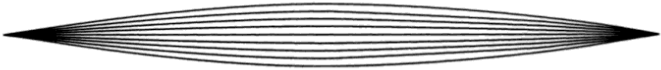
\includegraphics[width=\textwidth]{Assets/images/Onda_t}
					\label{Onda_t}}	
			\end{subfigure}
			\vspace{1cm}
			\begin{subfigure}
				[Oscilaciones de frecuencia 2F(Octava)]{
					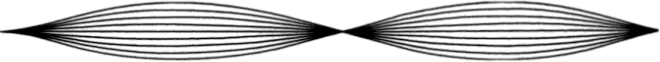
\includegraphics[width=\textwidth]{Assets/images/Onda_2t}
					\label{Onda_t2}}	
			\end{subfigure}
			\vspace{1cm}
			\begin{subfigure}
				[Oscilaciones de frecuencia 3F(Quinta)]{
					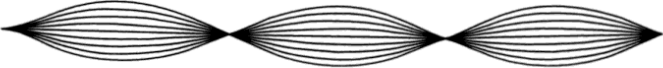
\includegraphics[width=\textwidth]{Assets/images/Onda_3t}
					\label{Onda_t3}}	
			\end{subfigure}
			\vspace{1cm}
			\caption{Escala Pitagórica ~\citep[p.~11]{musichistory}}
			\label{Pitagoras-scale}
		\end{center}    
	\end{figure}
	\pagebreak 
	Por el momento, nos conformaremos con llamar a esta frecuencia como F, es decir, la Fundamental pues resuena con todo el sistema aprovechando la mayor parte de la energía en su señal. Esto, producirá las perturbaciones en el medio que conoceremos como sonido, pues a diferencia del ruido, conocemos como está compuesta. Y este ruido será audible para el ser humano aproximadamente desde los 20 - 20,000[Hz] \citep[p.~16]{lopez2017diseno} entre tonos agudos, medios y graves.\par 
	
	Si bien, la cantidad de sonidos disponibles por las limitaciones físicas es muy amplia, solo nos interesan algunos valores específicos, especialmente aquellos que cuenten con una relación que permita la armonía sonora, es decir, que puedan interactuar sin ocupar las mismas frecuencias y estos sean agradables al oído.\par 
	
	Por ello y considerando una época donde los instrumentos no contaban con una gran precisión, además de un sistema métrico complejo, estos se relacionaban mediante fracciones del doble y triple, en cuanto a longitud de nuestra cuerda hipotética, como a esta no podemos modificar su tamaño, aún es posible controla la frecuencia, por lo que si duplicamos en valor de F, obtenemos la figura \ref{Onda_t2} donde se representan 2 nodos, el valor de 2F representará nuestro primer armónico con respecto a la fundamental.\\
	Si pudiésemos escuchar un sonido proveniente de ambos esquemas mencionados, ejecutados al mismo tiempo, percibiríamos el mismo Tono aunque a diferente escala. Pues siempre que se presente una relación con $f * 2^{n}$ donde \emph{n} es la escala con respecto al origen; estos sonidos serán parecidos aunque NO  aportarán una diversidad en relaciones sonoras.\par 
	
	Por otra parte, si establecemos otra relación de proporciones. Con tan solo el valor 3 como base de la relación, obtenemos algo de progreso, pues este cambio en la frecuencia si otorga ua diversidad sonora y en armonía. Como lo muestra en la figura \ref{Onda_t3}, esta relación cuenta con una distribución distinta en sus nodos, por lo que no podemos llamarlos armónicos, aunque siguen compartiendo una buena interacción.\\ 
	Entendiendo este contexto, ahora contamos con las herramientas para generar escalas de tonos relacionados. Para muestra, sigamos con el siguiente ejercicio: \\
	Comencemos partiendo de nuestra frecuencia F, al duplicarla, obtenemos su Octava, delimitando el espacio para colocar los tonos que originemos. Tomando en cuenta el hecho que las escalas solo varían en lo agudo ó grave que puedan sonar un mismo tono, nos encargaremos de llevar a este espectro de relación entre octavas y quintas. Vamos a adelantarnos y llamaremos al tono de nuestra frecuencia fundamental como Do, si multiplicamos por 3, es decir, obtenemos su primera quinta, claramente esto se saldría de nuestras delimitaciones, por tanto, dividiremos entre 2. Pues estamos usando la octava de esta quinta, pues hemos establecido que toda relación entre potencias con base 2 ocupan el mismo Tono.\par
	Esta quinta, la llamaremos Sol y repetiremos el proceso. Aunque de continuar, terminaríamos con una fracción mayor que 2F, por lo que debemos dividirla nuevamente entre 2. Este caso debe repetirse siempre que el número sea mayor igual que 2.\\
	Realizaremos una última observación al llegar con el tono Fa\#, este último no cuenta con un nombre propio, pero si es utilizado por lo que al estar un semitono arriba de la nota Fa, indicaremos su estado con el símbolo \emph{hash}.\pagebreak
	Así como pudimos obtener una relación con las quintas más agudas, podemos hacer lo mismo con los valores más bajos, dividiendo entre 3, aunque esto claramente nos dejaría fuera de nuestros límites, así que usaremos la octava para multiplicar por 2, así objetemos los Semitonos y tono restantes, siendo un énfasis en como este también pudo concluir con un valor muy cercano a la relación de frecuencia, si convertimos a decimal, existe una diferencia en centésimas con respecto relación de frecuencia. Por lo que podemos dar por cerrada esta escala denominada como Cromática. Aquella usada por la cultura occidental para componer e interpretar melodías.\par
	\begin{figure}[!b]
		\begin{center}
			
\includegraphics[width=\textwidth]{Assets/images/Stern-Brocot}
			\caption{Esquema inspirado en el Árbol Stern-Brocot.~\cite{teoriasescalas2013}}
			\label{Stern-Brocot}
		\end{center}
	\end{figure}
	\pagebreak
	Así es como obtenemos las escalas pentatónica, septuatónica y dodecatónica, siendo estas últimas 2 las más relevantes en el estudio y creación de la música. Aquellos primeros 7 tonos los cuales fueron nombrados con las Etiquetas \emph{Do, Re, Mi, Fa, Sol, La, Si}, así como algunos semitonos que se encuentran en medio de estos tonos para complementar la variedad de sonidos acordados.\par 
	Todavía debemos afinar un pequeño detalle, pues no hemos definido nuestra frecuencia F, de la cual solo hemos obtenido las relaciones...\\
	Históricamente, la nota utilizada para afinar el resto, ha sido "\emph{LA}" asignando una frecuencia de \textbf{440[Hz]}, tal modo que nos resulta una notación así:
	\begin{figure}[!b]
		\begin{center}
			
\includegraphics[width=\textwidth]{Assets/images/Stern-Brocot_resultados}
			\caption{Resultados de la escala Pitagórica}
			\label{res-pit}
		\end{center}
	\end{figure}\pagebreak
	Añadiendo el valor a F, obtenemos los siguientes resultados:
	\begin{figure}[!b]
		\begin{center}
			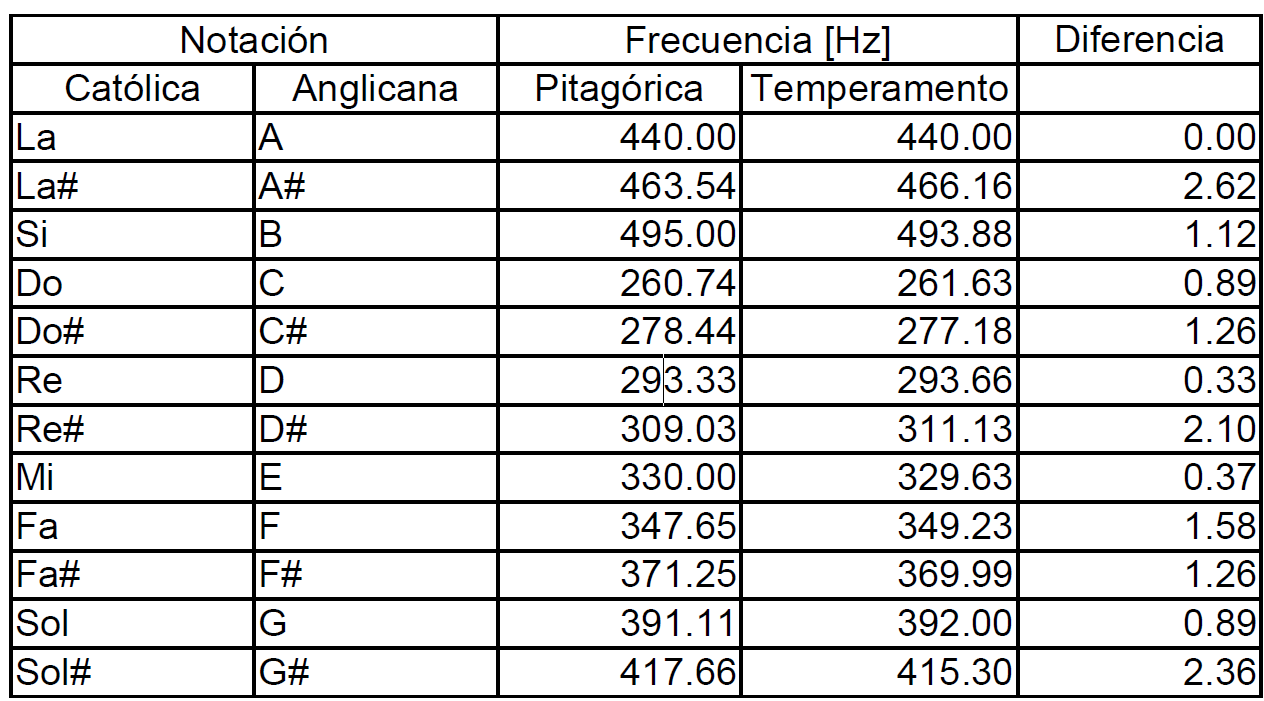
\includegraphics[width=\textwidth]{Assets/images/cmp}
			\caption{Comparación entre método pitagórico y consistente}
			\label{comp-pit}
		\end{center}
	\end{figure}
	\markboth{Análisis y Procesamiento de Audio}{Análisis y Procesamiento de Audio}
	\section*{Análisis y Procesamiento de Audio}\addcontentsline{toc}{section}{Análisis y Procesamiento de Audio}
	\subsection*{Definición Técnica del Audio}\addcontentsline{toc}{subsection}{Definición Técnica del Audio}
	\subsection*{Captura de Información}\addcontentsline{toc}{subsection}{Captura de Información}
	\subsection*{Procesamiento de Señal}\addcontentsline{toc}{subsection}{Procesamiento de Señal}
	\subsection*{Métodos de Aproximación}\addcontentsline{toc}{subsection}{Métodos de Aproximación}
	\section*{Construcción del NoiseMachine}\addcontentsline{toc}{section}{Construcción del NoiseMachine}
	\subsection*{Estudio del Proyecto olcSynth}\addcontentsline{toc}{subsection}{Estudio del Proyecto olcSynth}
	\subsection*{Aporte de Propuesta}\addcontentsline{toc}{subsection}{Aporte de Propuesta}
	\subsection*{Cambios y Pruebas del Software}\addcontentsline{toc}{subsection}{Cambios y Pruebas del Software}
	\subsection*{Implementación y Proyecciones a Futuro}\addcontentsline{toc}{subsection}{Implementación y Proyecciones a Futuro}
	\section*{Construcción del Tuner}\addcontentsline{toc}{section}{Construcción del Tuner}
	\subsection*{Estrategia y Diseño}\addcontentsline{toc}{subsection}{Estrategia y Diseño}
	\subsection*{Manejo de Excepciones}\addcontentsline{toc}{subsection}{Manejo de Excepciones}
	\subsection*{Capacidades Fundamentales}\addcontentsline{toc}{subsection}{Capacidades Fundamentales}
	\subsection*{Oportunidades de Innovación}\addcontentsline{toc}{subsection}{Oportunidades de Innovación}
	\section*{Diseño de los Instrumentos Virtuales}\addcontentsline{toc}{section}{Diseños de los Instrumentos Virtuales}
	\subsection*{Resumen de XML}\addcontentsline{toc}{subsection}{Resumen de XML}
	\subsection*{Propuesta de Convención}\addcontentsline{toc}{subsection}{Propuesta de Convención}
	\subsection*{Proyecciones con musicC++}\addcontentsline{toc}{subsection}{Proyecciones con musiC++}
	\subsection*{Comparación contra Formatos Estandarizados}\addcontentsline{toc}{subsection}{Comparación contra Formatos Estandarizados}
	\section*{Guía de Usuario}\addcontentsline{toc}{section}{Guía de Usuario}
	\subsection*{Paso 1: Recolección de Muestra}\addcontentsline{toc}{subsection}{Paso 1: Recolección de Muestra}
	\subsection*{Paso 2: Afinar el Instrumento Virtual}\addcontentsline{toc}{subsection}{Paso 2: Afinar el Instrumento Virtual}
	\subsection*{Paso 3: Prueba de Sonido}\addcontentsline{toc}{subsection}{Paso 3: Prueba de Sonido}
	\subsection*{Paso 4: Exportación a otros Productos}\addcontentsline{toc}{subsection}{Paso 4: Exportación a otros Productos}
	\section*{Conclusiones}\addcontentsline{toc}{section}{Conclusiones}
	\bibliography{Assets/ref/referencias}\addcontentsline{toc}{section}{Bibliografía}
	\section*{Anexos}\addcontentsline{toc}{section}{Anexos}
\end{document}

